% !TeX program = lualatex
% ================================================================
% Polish Parallel Text Version of StandardFormRevision
%
% Generated by the server using the following settings:
%
%   language            Polish (pol)
%   text direction      left to right
%   font                Noto Serif
%   fallback font       Noto Serif
%   built from          latex/worksheets/revision/standardFormRevision.tex
%   vocabulary key      latex/worksheets/revision/standardFormRevision/L2/pol/standardFormRevision_polishKey.tex
%   tier 3 vocabulary   green   RGB 0 128 0
%   English text        black   RGB 0 0 0
%   Polish text         purple  RGB 112 48 160
%   layout macros       version 3
%
% Please don't edit any information in this comment block - the server
% compares it against the current settings and rebuilds this file when
% they differ, so changes here would be overwritten. However, feel free
% to make updates to the LaTeX below if you want to edit it.
% ================================================================

\documentclass[11pt,a4paper]{article}
% ================================================================
% Copied from the English sheet this was translated from, so that
% anything it sets up for itself still works here
% ================================================================
\usepackage[a4paper,top=14mm,bottom=14mm,left=15mm,right=15mm]{geometry}
\usepackage[T1]{fontenc}
\usepackage{amsmath}
\usepackage{amssymb}
\usepackage{array}
\usepackage{multicol}
\usepackage{tikz}
\usetikzlibrary{arrows.meta}

% ================================================================
% Standard form: revision questions.
%
% Two pages of questions, in black and white, with a heading for each
% topic on the Maths Revision topic list in the same order. Each topic
% has a few short questions that start easy, with a diagram only where
% a question uses one, and the sheet ends with some problem solving.
% There are no key facts or worked examples on the sheet: the methods
% are in the worked solutions and the revision guide. Questions are
% numbered through the sheet so that the answer key and the worked
% solutions can refer to them.
% ================================================================

\pagestyle{empty}
\setlength{\parindent}{0pt}
\setlength{\parskip}{2pt}
\setlength{\columnsep}{9mm}

% A topic from the revision list.
\newcommand{\topic}[1]{\par\addvspace{9pt}{\bfseries #1}\par\nobreak\vspace{2pt}}

% Questions are numbered through the whole sheet.
\newcounter{qn}
\newcommand{\q}{\par\addvspace{5pt}\stepcounter{qn}\hangindent=1.6em\hangafter=1\noindent
  \makebox[1.6em][l]{\textbf{\theqn}}}

% A calculator key, drawn as a small box.
\newcommand{\calckey}[1]{{\setlength{\fboxsep}{1.5pt}\fbox{\small #1}}}

% Characters this language's font has not got are borrowed from another,
% rather than being silently dropped - see docs/translated-sheet-latex.md
\directlua{%
  if luaotfload and luaotfload.add_fallback then
    luaotfload.add_fallback("eallatinfallback",
      { "Noto Serif:mode=harf;" })
  else
    tex.error("this luaotfload is too old to register a fallback font")
  end
}
\usepackage[english]{babel}
\babelprovide[import]{polish}
\babelfont[polish]{rm}[Renderer=Harfbuzz, BoldFont={Noto Serif}, ItalicFont={Noto Serif}, BoldItalicFont={Noto Serif}, RawFeature={fallback=eallatinfallback}]{Noto Serif}
\babelfont[polish]{sf}[Renderer=Harfbuzz, BoldFont={Noto Serif}, ItalicFont={Noto Serif}, BoldItalicFont={Noto Serif}, RawFeature={fallback=eallatinfallback}]{Noto Serif}
\newcommand{\ealtext}[1]{\foreignlanguage{polish}{#1}}
\newcommand{\ealtextblock}[1]{{\raggedright\foreignlanguage{polish}{#1}\par}}
% ================================================================
% EAL layout helpers
% ================================================================
\usepackage{xcolor}

\definecolor{ealkeycolour}{RGB}{0,128,0}
\definecolor{ealenglish}{RGB}{0,0,0}
\definecolor{ealtwocolour}{RGB}{112,48,160}

\newsavebox{\ealboxen}
\newsavebox{\ealboxtr}
\newlength{\ealglosswd}
\newlength{\ealglossraise}
\setlength{\ealglossraise}{1.15em}

% a tier 3 word, in English and in translation alike
\newcommand{\ealkey}[1]{\textcolor{ealkeycolour}{#1}}
\newcommand{\ealkeytr}[1]{\textcolor{ealkeycolour}{\ealtext{#1}}}

% One translated word above one English word. Built from kernel
% primitives, never a tabular, which would break wherever the sheet
% loads array, booktabs or tabularx. The box is as wide as the wider of
% the two, so a long translation pushes its neighbours aside instead of
% overlapping them, and it claims its full height so a table row or a
% TikZ node makes room for it.
\newcommand{\ealgloss}[2]{%
  \sbox{\ealboxen}{\ealkey{#1}}%
  \sbox{\ealboxtr}{\small\textcolor{ealtwocolour}{\ealtext{#2}}}%
  \setlength{\ealglosswd}{\wd\ealboxen}%
  \ifdim\wd\ealboxtr>\ealglosswd\setlength{\ealglosswd}{\wd\ealboxtr}\fi
  \leavevmode
  \makebox[\ealglosswd][c]{%
    \makebox[0pt][c]{\usebox{\ealboxen}}%
    \makebox[0pt][c]{\raisebox{\ealglossraise}{\usebox{\ealboxtr}}}%
  }%
}

% opens up line spacing around a block of glosses, so the raised
% translations sit clear of the line above
\newenvironment{ealglossed}{\par\linespread{2.1}\selectfont\ignorespaces}{\par}

% a whole translated sentence above its English counterpart. block level,
% so it does not belong inside a tabular cell
\newcommand{\ealpara}[2]{%
  \par\addvspace{0.5\baselineskip}%
  {\color{ealtwocolour}\ealtextblock{#1}}%
  \penalty200
  {\color{ealenglish}#2\par}%
  \addvspace{0.5\baselineskip}%
}

\begin{document}
% Ragged right, without \raggedright, which would make \\ end the
% paragraph and lose the hanging indent of a question's later lines.
\setlength{\rightskip}{0pt plus 4em}

{\Large\bfseries \ealkey{Standard form}}\hfill{\large Revision questions}
\par\vspace{2pt}\hrule\vspace{4pt}

\begin{multicols}{2}

% ----------------------------------------------------------------
\ealpara{Zapisywanie dużych i małych liczb w \ealkeytr{notacji naukowej}}{Writing large and small numbers in \ealkey{standard form}}
\topic{Writing large and small numbers in \ealkey{standard form}}
\ealpara{Tabela \ealkeytr{wartości pozycyjnych} pokazuje liczbę 72\,500. Zapisz 72\,500 w \ealkeytr{notacji naukowej}.}{The \ealkey{place value} table shows the number 72\,500. Write 72\,500 in \ealkey{standard form}.}
\q The \ealkey{place value} table shows the number 72\,500. Write 72\,500 in \ealkey{standard form}.\\[4pt]
{\renewcommand{\arraystretch}{1.5}%
\begin{tabular}{|c|c|c|c|c|}\hline
$10^4$ & $10^3$ & $10^2$ & $10^1$ & $10^0$\\\hline
7 & 2 & 5 & 0 & 0\\\hline
\end{tabular}}
\ealpara{Zapisz w \ealkeytr{notacji naukowej}.}{Write in \ealkey{standard form}.}
\q Write in \ealkey{standard form}.\\
(a) 6000\qquad (b) 3\,080\,000\\
(c) 0.009\qquad (d) 0.000\,304
\ealpara{Zapisz jako \ealkeytr{liczby w zwykłej postaci}.}{Write as \ealkey{ordinary numbers}.}
\q Write as \ealkey{ordinary numbers}.\\
(a) $3\times10^6$\qquad (b) $2.07\times10^4$\\
(c) $5\times10^{-2}$\qquad (d) $6.1\times10^{-5}$
\ealpara{Dwie z tych liczb nie są zapisane w \ealkeytr{notacji naukowej}. Znajdź je i zapisz je poprawnie.}{Two of these numbers are not written in \ealkey{standard form}. Find them, and write them correctly.}
\q Two of these numbers are not written in \ealkey{standard form}. Find them, and write them correctly.
\[ 34\times10^5\qquad 7\times10^{-2}\qquad 0.7\times10^3\qquad 1.5\times10^9 \]
\ealpara{Planeta Merkury znajduje się około 58\,000\,000\,km od Słońca. Zapisz tę odległość w \ealkeytr{notacji naukowej}.}{The planet Mercury is about 58\,000\,000\,km from the Sun. Write this distance in \ealkey{standard form}.}
\q The planet Mercury is about 58\,000\,000\,km from the Sun. Write this distance in \ealkey{standard form}.
\ealpara{Tabela pokazuje szerokości niektórych małych rzeczy. Zapisz je w kolejności od najmniejszej do największej.}{The table shows the widths of some small things. Write them in order, smallest first.}
\q The table shows the widths of some small things. Write them in order, smallest first.\\[4pt]
{\renewcommand{\arraystretch}{1.5}%
\begin{tabular}{|l|c|}\hline
Grain of sand & $5\times10^{-4}$ m\\\hline
Human hair & $7\times10^{-5}$ m\\\hline
Red blood cell & $8\times10^{-6}$ m\\\hline
Ant & $4\times10^{-3}$ m\\\hline
\end{tabular}}
\ealpara{Ziarno piasku \quad Włos ludzki \quad Czerwona krwinka \quad Mrówka}{Grain of sand \quad Human hair \quad Red blood cell \quad Ant}

% ----------------------------------------------------------------
\ealpara{Mnożenie i dzielenie w \ealkeytr{notacji naukowej}}{\ealkey{Multiplying} and \ealkey{dividing} in \ealkey{standard form}}
\topic{\ealkey{Multiplying} and \ealkey{dividing} in \ealkey{standard form}}
\ealpara{Oblicz, podając odpowiedzi w \ealkeytr{notacji naukowej}.}{Work out, giving your answers in \ealkey{standard form}.}
\q Work out, giving your answers in \ealkey{standard form}.\\[2pt]
(a) $(2\times10^3)\times(4\times10^5)$\\[2pt]
(b) $(5\times10^6)\times(3\times10^{-2})$\\[2pt]
(c) $(9\times10^8)\div(3\times10^2)$\\[2pt]
(d) $(2\times10^{-3})\div(8\times10^4)$
\ealpara{Kartka papieru ma grubość $1\times10^{-4}$\,m. Jak wysoki jest stos $5\times10^3$ kartek? Podaj odpowiedź w \ealkeytr{notacji naukowej}.}{A sheet of paper is $1\times10^{-4}$\,m thick. How tall is a pile of $5\times10^3$ sheets? Give your answer in \ealkey{standard form}.}
\q A sheet of paper is $1\times10^{-4}$\,m thick. How tall is a pile of $5\times10^3$ sheets? Give your answer in \ealkey{standard form}.
\ealpara{Światło przebywa $3\times10^5$\,km w ciągu jednej sekundy. Jaką odległość przebywa światło w ciągu $2\times10^3$ sekund?}{Light travels $3\times10^5$\,km in one second. How far does light travel in $2\times10^3$ seconds?}
\q Light travels $3\times10^5$\,km in one second. How far does light travel in $2\times10^3$ seconds?

% ----------------------------------------------------------------
\ealpara{Dodawanie i odejmowanie w \ealkeytr{notacji naukowej}}{\ealkey{Adding} and \ealkey{subtracting} in \ealkey{standard form}}
\topic{\ealkey{Adding} and \ealkey{subtracting} in \ealkey{standard form}}
\ealpara{Oblicz, podając odpowiedzi w \ealkeytr{notacji naukowej}.}{Work out, giving your answers in \ealkey{standard form}.}
\q Work out, giving your answers in \ealkey{standard form}.\\[2pt]
(a) $6\times10^4+3\times10^3$\\[2pt]
(b) $8.5\times10^6-4\times10^5$\\[2pt]
(c) $2\times10^{-3}+6\times10^{-4}$\\[2pt]
(d) $7\times10^{-2}-5\times10^{-3}$
\ealpara{Ben mówi: „$3\times10^4+2\times10^3=5\times10^7$.” Wyjaśnij błąd Bena i znajdź poprawną odpowiedź.}{Ben says, ``$3\times10^4+2\times10^3=5\times10^7$.'' Explain Ben's mistake, and find the correct answer.}
\q Ben says, ``$3\times10^4+2\times10^3=5\times10^7$.'' Explain Ben's mistake, and find the correct answer.
\ealpara{\ealkeytr{Średnica} Jowisza wynosi $1.43\times10^5$\,km. \ealkeytr{Średnica} Ziemi wynosi $1.27\times10^4$\,km. O ile większa jest \ealkeytr{średnica} Jowisza? Podaj odpowiedź w \ealkeytr{notacji naukowej}.}{The \ealkey{diameter} of Jupiter is $1.43\times10^5$\,km. The \ealkey{diameter} of the Earth is $1.27\times10^4$\,km. How much bigger is the \ealkey{diameter} of Jupiter? Give your answer in \ealkey{standard form}.}
\q The \ealkey{diameter} of Jupiter is $1.43\times10^5$\,km. The \ealkey{diameter} of the Earth is $1.27\times10^4$\,km. How much bigger is the \ealkey{diameter} of Jupiter? Give your answer in \ealkey{standard form}.

\end{multicols}

\newpage

\begin{multicols}{2}

% ----------------------------------------------------------------
\ealpara{\ealkeytr{Notacja naukowa} z kalkulatorem}{\ealkey{Standard form} with a calculator}
\topic{\ealkey{Standard form} with a calculator}
\ealpara{Użyj kalkulatora. Podaj odpowiedzi w \ealkeytr{notacji naukowej}.}{Use a calculator. Give your answers in \ealkey{standard form}.}
\q Use a calculator. Give your answers in \ealkey{standard form}.\\[2pt]
(a) $(6.3\times10^7)\times(4.8\times10^{-3})$\\[2pt]
(b) $(7.5\times10^4)^2$\\[2pt]
(c) $(9.6\times10^5)\div(1.2\times10^{-3})$\\[2pt]
(d) $\sqrt{4.9\times10^7}$\\[4pt]
\ealpara{Na większości kalkulatorów \ealkeytr{notację naukową} wprowadza się za pomocą klawisza \calckey{$\times10^x$}.}{On most calculators, \ealkey{standard form} is entered with the \calckey{$\times10^x$} key.}
\ealpara{Ava chce obliczyć $(4\times10^3)\div(2\times10^2)$. Wpisuje \calckey{4} \calckey{$\times$} \calckey{1} \calckey{0} \calckey{$x^\square$} \calckey{3} \calckey{$\div$} \calckey{2} \calckey{$\times$} \calckey{1} \calckey{0} \calckey{$x^\square$} \calckey{2} \calckey{$=$} i otrzymuje 200\,000. Poprawna odpowiedź to 20. Wyjaśnij, co poszło nie tak.}{Ava wants to work out $(4\times10^3)\div(2\times10^2)$. She types \calckey{4} \calckey{$\times$} \calckey{1} \calckey{0} \calckey{$x^\square$} \calckey{3} \calckey{$\div$} \calckey{2} \calckey{$\times$} \calckey{1} \calckey{0} \calckey{$x^\square$} \calckey{2} \calckey{$=$} and gets 200\,000. The correct answer is 20. Explain what has gone wrong.}
\q Ava wants to work out $(4\times10^3)\div(2\times10^2)$. She types\\[3pt]
\calckey{4} \calckey{$\times$} \calckey{1} \calckey{0} \calckey{$x^\square$} \calckey{3} \calckey{$\div$} \calckey{2} \calckey{$\times$} \calckey{1} \calckey{0} \calckey{$x^\square$} \calckey{2} \calckey{$=$}\\[3pt]
and gets 200\,000. The correct answer is 20. Explain what has gone wrong.

% ----------------------------------------------------------------
\ealpara{Zadania z \ealkeytr{notacją naukową}}{Problems with \ealkey{standard form}}
\topic{Problems with \ealkey{standard form}}
\ealpara{Księżyc znajduje się $3.84\times10^8$\,m od Ziemi. Światło porusza się z prędkością $3\times10^8$\,m na sekundę. Ile sekund potrzeba, aby światło z Księżyca dotarło do Ziemi?}{The Moon is $3.84\times10^8$\,m from the Earth. Light travels at $3\times10^8$\,m per second. How many seconds does light from the Moon take to reach the Earth?}
\q The Moon is $3.84\times10^8$\,m from the Earth. Light travels at $3\times10^8$\,m per second. How many seconds does light from the Moon take to reach the Earth?\\[4pt]
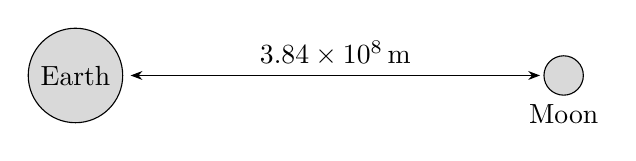
\begin{tikzpicture}[x=1mm,y=1mm]
  \draw[fill=black!15] (0,0) circle (6);
  \node at (0,0) {Earth};
  \draw[fill=black!15] (62,0) circle (2.5);
  \node[below=2.5mm] at (62,0) {Moon};
  \draw[{Stealth[length=1.5mm]}-{Stealth[length=1.5mm]}] (7,0) -- (59,0);
  \node[above] at (33,0) {$3.84\times10^8$\,m};
\end{tikzpicture}

\columnbreak
\ealpara{Statek kosmiczny porusza się z prędkością $1.1\times10^4$\,m na sekundę przez jedną godzinę, czyli $3.6\times10^3$ sekund. Jaką odległość przebywa? Podaj odpowiedź w \ealkeytr{notacji naukowej}.}{A spacecraft travels at $1.1\times10^4$\,m per second for one hour, which is $3.6\times10^3$ seconds. How far does it travel? Give your answer in \ealkey{standard form}.}
\q A spacecraft travels at $1.1\times10^4$\,m per second for one hour, which is $3.6\times10^3$ seconds. How far does it travel? Give your answer in \ealkey{standard form}.
\ealpara{Czerwona krwinka ma szerokość $8\times10^{-6}$\,m. Ile czerwonych krwinek zmieściłoby się obok siebie wzdłuż paznokcia o szerokości $2\times10^{-2}$\,m?}{A red blood cell is $8\times10^{-6}$\,m wide. How many red blood cells would fit side by side across a fingernail $2\times10^{-2}$\,m wide?}
\q A red blood cell is $8\times10^{-6}$\,m wide. How many red blood cells would fit side by side across a fingernail $2\times10^{-2}$\,m wide?
\ealpara{Liczba ludności Wielkiej Brytanii wynosi około $6.8\times10^7$. \ealkeytr{Pole} Wielkiej Brytanii wynosi około $2.4\times10^5$\,km$^2$. Jaka jest \ealkeytr{średnia} liczba osób przypadających na każdy km$^2$? Podaj odpowiedź z dokładnością do 2 \ealkeytr{cyfr znaczących}.}{The population of the UK is about $6.8\times10^7$. The \ealkey{area} of the UK is about $2.4\times10^5$\,km$^2$. On \ealkey{average}, how many people are there for each km$^2$? Give your answer to 2 \ealkey{significant figures}.}
\q The population of the UK is about $6.8\times10^7$. The \ealkey{area} of the UK is about $2.4\times10^5$\,km$^2$. On \ealkey{average}, how many people are there for each km$^2$? Give your answer to 2 \ealkey{significant figures}.
\ealpara{Masa Ziemi wynosi $5.97\times10^{24}$\,kg. Masa Księżyca wynosi $7.35\times10^{22}$\,kg. Ile razy Ziemia jest cięższa od Księżyca? Podaj odpowiedź z dokładnością do najbliższej \ealkeytr{liczby całkowitej nieujemnej}.}{The mass of the Earth is $5.97\times10^{24}$\,kg. The mass of the Moon is $7.35\times10^{22}$\,kg. How many times heavier is the Earth than the Moon? Give your answer to the nearest \ealkey{whole number}.}
\q The mass of the Earth is $5.97\times10^{24}$\,kg. The mass of the Moon is $7.35\times10^{22}$\,kg. How many times heavier is the Earth than the Moon? Give your answer to the nearest \ealkey{whole number}.

% ----------------------------------------------------------------
\ealpara{Rozwiązywanie problemów}{Problem solving}
\topic{Problem solving}
\ealpara{Komputer wykonuje $3\times10^9$ obliczeń każdą sekundę. Ile godzin potrzeba na wykonanie $1.2\times10^{14}$ obliczeń? Podaj odpowiedź z dokładnością do 1 \ealkeytr{miejsca dziesiętnego}.}{A computer does $3\times10^9$ calculations each second. How many hours does it take to do $1.2\times10^{14}$ calculations? Give your answer to 1 \ealkey{decimal place}.}
\q A computer does $3\times10^9$ calculations each second. How many hours does it take to do $1.2\times10^{14}$ calculations? Give your answer to 1 \ealkey{decimal place}.
\ealpara{Dwie liczby w \ealkeytr{notacji naukowej} są \ealkeytr{mnożone}, a wynik wynosi $6\times10^5$. Zapisz trzy różne pary liczb, które mogły być \ealkeytr{mnożone}.}{Two numbers in \ealkey{standard form} are \ealkey{multiplied}, and the answer is $6\times10^5$. Write down three different pairs of numbers that could have been \ealkey{multiplied}.}
\q Two numbers in \ealkey{standard form} are \ealkey{multiplied}, and the answer is $6\times10^5$. Write down three different pairs of numbers that could have been \ealkey{multiplied}.
\ealpara{Co jest większe: $(2\times10^3)^3$ czy $10^{10}$? Pokaż, skąd to wiesz.}{Which is bigger, $(2\times10^3)^3$ or $10^{10}$? Show how you know.}
\q Which is bigger, $(2\times10^3)^3$ or $10^{10}$? Show how you know.

\end{multicols}

\end{document}